\section{Implementation and Results}
  \subsection{Coefficient of Model 2}
    \par We produced the result of Model 2 with 4 different values of $\gamma$:
    \begin{itemize}
      \item $10\%$ (\texttt{model2-1})
      \item $25\%$ (\texttt{model2-2})
      \item $40\%$ (\texttt{model2-3})
      \item $50\%$ (\texttt{model2-4})
    \end{itemize}

  \subsection{Programming Language and Library}
    \par The two models mentioned in section 2 are implemented using Python 3. The library that we used to solve Linear Optimization is \href{https://www.mosek.com/}{\texttt{MOSEK}}.

  \subsection{Implementation Issues}
    \par Out of 133 transactions in the dataset, model 1 successfully solved all. Meanwhile, model 2 failed on a few transactions (from 1 to 4 transactions out of 133, according to different values of $\gamma$). The unsolved transactions often have really large number of inputs (more than 19.000). Some transaction was successfully solved with a particular value of $\gamma$ but was unsolved with another value. Based on our observation, as well as the \texttt{MOSEK} documentation, we suspect the unsolved transactions are caused by numerical issues.
    \par To get the full result despite the unsolved transactions of model 2, for each unsolved transaction we will use the result of model 1 instead, since the result of model 1 is one viable solution of model 2.

  \subsection{Results}
    \par The result of the two models is visualized with the following charts.
    \subsubsection{Transaction Size}
      \begin{figure}[H]
        \center{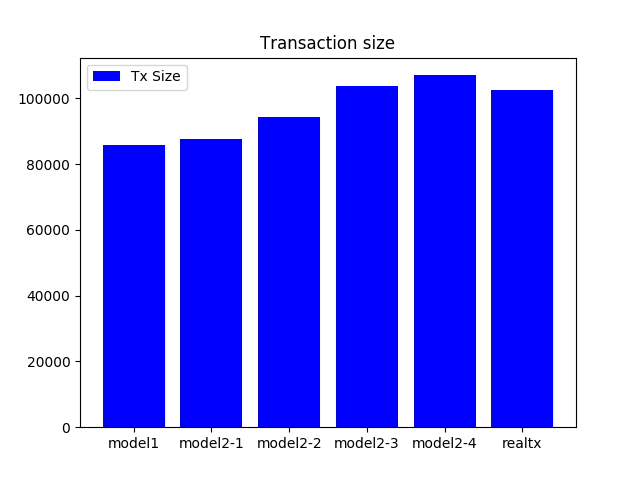
\includegraphics[width=12.5cm]
        {plot01.png}}
      \end{figure}
    \subsubsection{Number of Selected UTXOs}
      \begin{figure}[H]
        \center{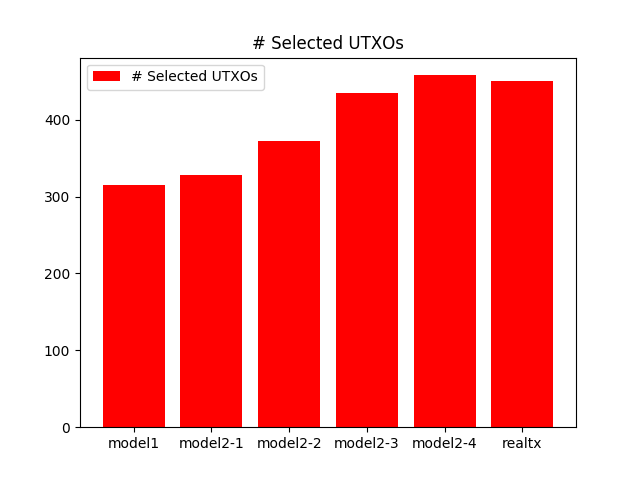
\includegraphics[width=12.5cm]
        {plot02.png}}
      \end{figure}
    \subsubsection{Average Value of Selected UTXOs}
      \begin{figure}[H]
        \center{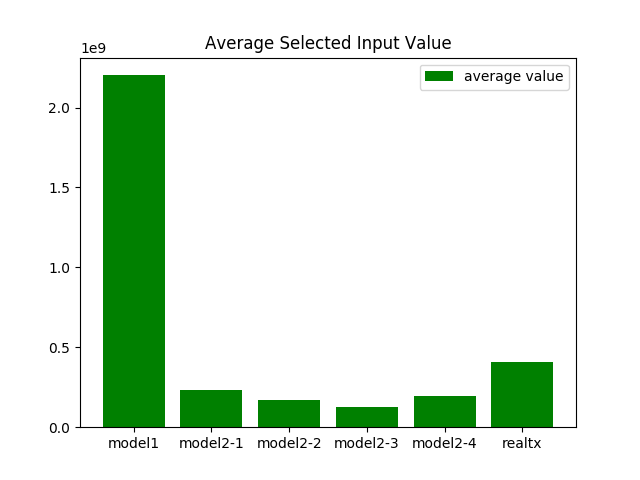
\includegraphics[width=12.5cm]
        {plot03.png}}
      \end{figure}
